
Table Basic concepts for types and objects lists the basic concepts for types and objects in general.

Table Concepts for ranges, iterators, and algorithms lists the concepts for ranges, views, iterators, and algorithms.

Table Auxiliary concepts lists the concepts that are used mainly as building blocks for other concepts and are usually not used directly by application programmers.

\subsubsection*{\zihao{3} 5.1.1\hspace{0.2cm}Header Files and Namespaces}
\addcontentsline{toc}{subsubsection}{5.1.2\hspace{0.2cm}Header Files and Namespaces}

Standard concepts are defined in different header files:

\begin{itemize}
\item
Many basic concepts are defined in the header file <concepts>, which is included by <ranges> and <iterator>.

\item
Concepts for iterators are defined in the header file <iterator>.

\item
Concepts for ranges are defined in the header file <ranges>.

\item
three\_way\_comparable concepts are defined in <compare> (which is included by almost every other header file).

\item
uniform\_random\_bit\_generator is defined in <random>.
\end{itemize}

Almost all concepts are defined in the namespace std. The only exceptions to this rule are the ranges concepts, which are defined in the namespace std::ranges.

\begin{table}[H]
\centering
\begin{tabular}{|l|l|}
	\hline
	\textbf{Concept} &
	\textbf{Constraint} \\ \hline
	\begin{tabular}[c]{@{}l@{}}integral\\ signed\_integral\\ unsigned\_integral\\ floating\_point\end{tabular} &
	\begin{tabular}[c]{@{}l@{}}Integral type\\ Signed integral type\\ Unsigned integral type\\ Floating-point type\end{tabular} \\ \hline
	\begin{tabular}[c]{@{}l@{}}movable\\ copyable\\ semiregular\\ regular\end{tabular} &
	\begin{tabular}[c]{@{}l@{}}Supports move initialization/assignment and swaps\\ Supports move and copy initialization/assignment and swaps\\ Supports default initialization, copies, moves and swaps\\ Supports default initialization, copies, moves, swaps, and equality comparisons\end{tabular} \\ \hline
	\begin{tabular}[c]{@{}l@{}}same\_as\\ convertible\_to\\ derived\_from\\ constructible\_from\\ assigneable\_from\\ swappable\_with\\ common\_with\\ common\_reference\_with\end{tabular} &
	\begin{tabular}[c]{@{}l@{}}Same types\\ Type convertible to another type\\ Type derived from another type\\ Type constructiable from others types\\ Type assignable from another type\\ Type swappable with another type\\ Two types have a common type\\ Two types have a common reference type\end{tabular} \\ \hline
	\begin{tabular}[c]{@{}l@{}}equality\_comparable\\ equality\_comparable\_with\\ totally\_ordered\\ totally\_ordered\_with\\ three\_way\_comparable\\ three\_way\_comparable\_with\end{tabular} &
	\begin{tabular}[c]{@{}l@{}}Type supports checks for equality\\ Can check two types for equality\\ Types support a strict weak ordering\\ Can check two types for strict weak ordering\\ Can apply all comparison operators(includeing the operator\textless{}=\textgreater{})\\ Can compare two types with all comparison operators(including \textless{}=\textgreater{})\end{tabular} \\ \hline
	\begin{tabular}[c]{@{}l@{}}invocable\\ regular\_invocable\\ predicate\\ relation\\ equivalence\_relation\\ strict\_weak\_order\\ uniform\_random\_bit\_generator\end{tabular} &
	\begin{tabular}[c]{@{}l@{}}Type is a callable for specified arguments\\ Type is a callable for specified arguments(no modifications)\\ Type is a predicate(callable that returns a Boolean value)\\ A callable type defines a relationship between two types\\ A callable type defines an equality relationship between two types\\ A callable type defines an ordering relationship between two types\\ A callable type can be used as a random number generator\end{tabular} \\ \hline
\end{tabular}
\end{table}

\begin{center}
Table 5.1. Basic concepts for types and objects
\end{center}

\begin{table}[H]
\centering
\begin{tabular}{|l|l|}
	\hline
	\textbf{Concept} &
	\textbf{Constraint} \\ \hline
	\begin{tabular}[c]{@{}l@{}}default\_initializable\\ move\_constructible\\ copy\_constructible\\ destructible\\ swappable\\ weakly\_incrementables\\ incrementable\end{tabular} &
	\begin{tabular}[c]{@{}l@{}}Type is default initializable\\ Type supports move initializations\\ Type supports copy initializations\\ Type is destructible\\ Type is swappable\\ Type supports the increment operators\\ Type supports equality-preserving increment operator\end{tabular} \\ \hline
\end{tabular}
\end{table}

\begin{center}
Table 5.2. Auxiliary concepts
\end{center}

\begin{table}[H]
\begin{tabular}{|l|l|}
	\hline
	\textbf{Concept} &
	\textbf{Constraint} \\ \hline
	\begin{tabular}[c]{@{}l@{}}range\\ output\_range\\ input\_range\\ forward\_range\\ bidirectional\_range\\ random\_access\_range\\ contiguous\_range\\ sized\_range\\ common\_range\\ borrowed\_range\\ view\\ vieable\_range\end{tabular} &
	\begin{tabular}[c]{@{}l@{}}Type is a range\\ Type is a range to write to\\ Type is a range to read from\\ Type is a range to read from multiple times\\ Type is a range to read forward and backward from\\ Type is a range that supports jumping around over elements\\ Type is a range with elements in contiguous memory\\ Type is a range with cheap size support\\ Type is a range with iterators and sentinels that have the same type\\ Type is an lvalue or a borrowed range\\ Type is a view\\ Type is or can be converted to a view\end{tabular} \\ \hline
	\begin{tabular}[c]{@{}l@{}}indirectly\_writable\\ indirectly\_readable\\ indirectly\_movable\\ indirectly\_movable\_storable\\ indirectly\_copyable\\ indirectly\_copyable\_storable\\ indirectly\_swappable\\ indirectly\_comparable\end{tabular} &
	\begin{tabular}[c]{@{}l@{}}Type can be used to write to where it refers\\ Type can be used to read from where it refers\\ Type refers to movable objects\\ Type refers to movable objects with support for temporaries\\ Type refers to copyable objects\\ Type refers to copyable objects with support for temporaries\\ Type refers to swappable objects\\ Type refers to comparable objects\end{tabular} \\ \hline
	\begin{tabular}[c]{@{}l@{}}input\_output\_iterator\\ output\_iterator\\ input\_iterator\\ forward\_iterator\\ bidirectional\_iterator\\ random\_access\_iterator\\ contiguous\_interator\\ sentinel\_for\\ sized\_sentinel\_for\end{tabular} &
	\begin{tabular}[c]{@{}l@{}}Type is an iterator\\ Type is an output iterator\\ Type is (at least) an input iterator\\ Type is (at least) a forward iterator\\ Type is (at least) a bidirectional iterator\\ Type is (at least) a random-access iterator\\ Type is an iterator to elements in contiguous memory\\ Type can be used as a sentinel for an iterator type\\ Type can be used as a sentinel for an iterator type with cheap computaion of distance\end{tabular} \\ \hline
	\begin{tabular}[c]{@{}l@{}}permutable\\ mergeable\\ sortable\end{tabular} &
	\begin{tabular}[c]{@{}l@{}}Type is(at least) a forward iterator that can reorder elements\\ Two types can be used to merge sorted elements into a third type\\ A type is sortable(according to a comparison and projection)\end{tabular} \\ \hline
	\begin{tabular}[c]{@{}l@{}}indirectly\_unary\_invocable\\ indirectly\_regular\_unary\_invocable\\ indirect\_unary\_predicate\\ indirect\_binary\_predicate\\ indirect\_equivalence\_relation\\ indirect\_strict\_weak\_order\end{tabular} &
	\begin{tabular}[c]{@{}l@{}}Operation can be called with the value type of an iterator\\ Stateless operation can be called with the value types of an iterator\\ Unary predicate can be called with the value type of an iterator\\ Binary predicate can be called with the value types of two iterators\\ Predicate can be used to check two values of the passed iterator(s) for equality\\ Predicate can be used to order two values of the passed iterator(s)\end{tabular} \\ \hline
\end{tabular}
\end{table}

\begin{center}
Table 5.3. Concepts for ranges, iterators, and algorithms
\end{center}

\subsubsection*{\zihao{3} 5.1.2\hspace{0.2cm}Standard Concepts Subsume}
\addcontentsline{toc}{subsubsection}{5.1.2\hspace{0.2cm}Standard Concepts Subsume}

The concepts provided by the C++ standard library are carefully designed to subsume other concepts when this makes sense. In fact, they build a pretty complex subsumption graph. Figure 5.1 gives an impression of how complex it is.

\begin{center}
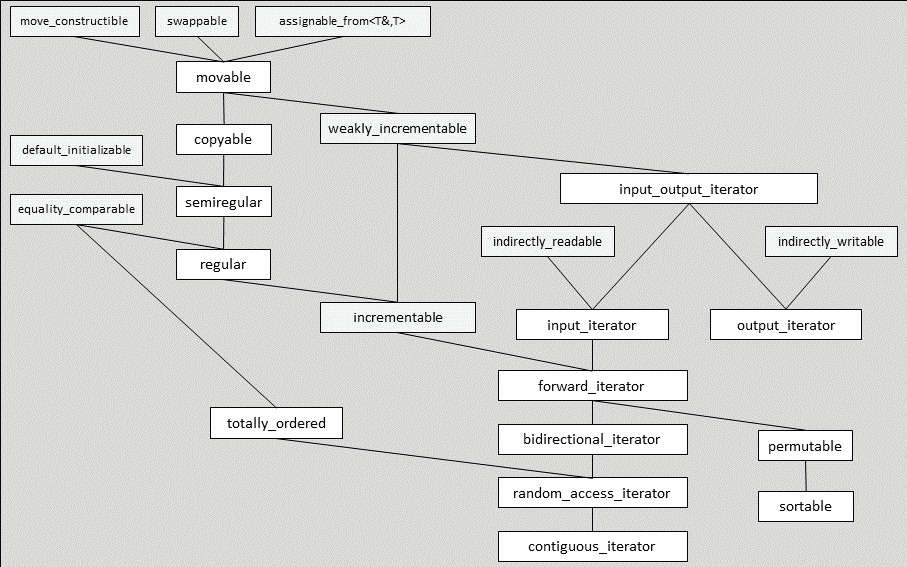
\includegraphics[width=1.\textwidth]{content/chapter5/images/1.png}\\
Figure 5.1. Subsumption graph of C++ standard concepts (extract)
\end{center}

For this reason, the description of the concepts lists which other key concepts are subsumed.



